\documentclass{beamer}
\usefonttheme[onlymath]{serif}
\usetheme[numbering=fraction, progressbar=frametitle]{metropolis}
\usepackage{appendixnumberbeamer}
\useoutertheme[footline=empty,subsection=false]{miniframes}
\useinnertheme{circles}
% \setbeamertemplate{headline}{%
%     \begin{beamercolorbox}[colsep=1.5pt]{upper separation line head}
%     \end{beamercolorbox}
%     \begin{beamercolorbox}{section in head/foot}
%     \vskip2pt\insertsectionnavigationhorizontal{\paperwidth}{}{}\vskip2pt
%         \end{beamercolorbox}%
%         \begin{beamercolorbox}[colsep=1.5pt]{lower separation line head}
%     \end{beamercolorbox}
% }


\usepackage[utf8]{inputenc}
\usepackage[T1]{fontenc}
\usepackage{textcomp}
\usepackage{amsmath, amssymb, amsthm}

\usepackage[style=authoryear,maxbibnames=9,maxcitenames=2,uniquelist=false,backend=biber,doi=false,url=false]{biblatex}
\renewcommand*{\nameyeardelim}{\addcomma\space} % have comma in parencite
\addbibresource{$BIB} % bibtex location
%%% Small bibliography slide
\setbeamertemplate{bibliography item}[triangle]
\makeatletter
\newcommand{\srcsize}{\@setfontsize{\srcsize}{6.5pt}{6.5pt}}
\makeatother
\renewcommand*{\bibfont}{\srcsize}

\usepackage{import}
\usepackage{pdfpages}
\usepackage{transparent}
\usepackage{xcolor}

\newcommand{\blue}[1]{\textcolor{blue}{#1}}
\newcommand{\red}[1]{\textcolor{red}{#1}}

\graphicspath{ {./figures} }
\newcommand{\inkfig}[2][1]{%
    \def\svgwidth{#1\columnwidth}
    \import{./figures/}{#2.pdf_tex}
}

%%%%%% Template
\usepackage{hyperref}
\definecolor{links}{HTML}{2A1B81}

%% beaver (red) style:
% \usecolortheme{beaver}
% \setbeamercolor{block body}{bg=gray!30!white}
% \setbeamercolor{block title}{bg=darkred!70, fg=black!2}
% \hypersetup{colorlinks=true,allcolors=red}

%% seahorse style:
\usecolortheme{seahorse}
\setbeamercolor{block body}{bg=mDarkTeal!30}
\setbeamercolor{block title}{bg=mDarkTeal,fg=black!2}
\hypersetup{colorlinks=true,allcolors=links}
%%%%%% Template

\pdfsuppresswarningpagegroup=1

\title{Review of Mathematics}
\author{\textit{Hui-Jun Chen}}
\date{\today}

\begin{document}

\maketitle

\section{Area Formula}%
\label{sec:area_formula}

\begin{frame}[t]{Area Formula: Triangle}
    \centering
    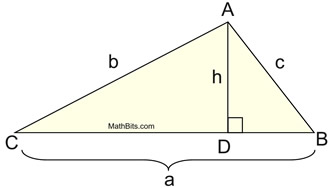
\includegraphics[width=0.5\textwidth]{./figures/triArea2.jpg}
    \begin{itemize}
        \item Area formula: $\frac{1}{2}  \times a  \times h$
    \end{itemize}
\end{frame}

\begin{frame}[t]{Area Formula: Rectangle}
    \centering
    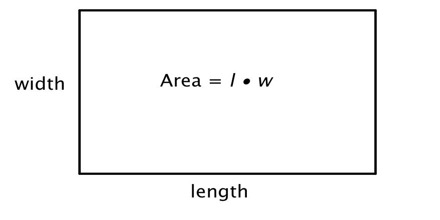
\includegraphics[width=0.7\textwidth]{./figures/qwe.jpg}
    \begin{itemize}
        \item Area formula: $length \times  width$
    \end{itemize}

\end{frame}

\begin{frame}[t]{Area Formula: Trapezoid}
    \centering
    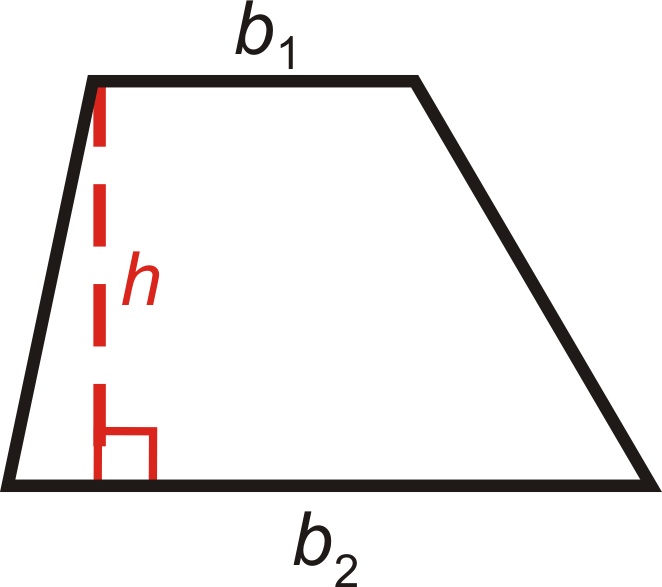
\includegraphics[width=0.4\textwidth]{./figures/trapezoid.png}
    \begin{itemize}
	\item Area formula: $\frac{\left( b_{1} + b_{2}  \right) }{2}  \times h$
	\item Or separate into two triangles and one rectangle
    \end{itemize}
\end{frame}


\section{Basic Algebra Review}%
\label{sec:basic_algebra_review}

\begin{frame}[t]{Basic Algebra Review: properties}
    \begin{itemize}
        \item Associative properties:
	    \begin{itemize}
		\item additive: $a + \left( b+c \right) = \left( a+b \right) +c$
		\item multiplicative: $a\left( bc \right) = \left( ab \right) c$
	    \end{itemize}
	\item Commutative properties:
	    \begin{itemize}
		\item additive: $a+b = b+a$
		\item multiplicative: $ab = ba$
	    \end{itemize}
	\item Distributive properties: $a\left( b+c \right) = ab + ac$
	\item Properties for exponents:
	    \begin{itemize}
	        \item $a^{x} a^{y} = a^{x+y} $; $\frac{a^{x} }{a^{y} } = a^{x-y} $
		\item $\left( ab \right)^{x} = a^{x} b^{x} $; $\left( \frac{a}{b}  \right)^{x} = \frac{a^{x} }{b^{x} } $
		\item $\left( a^{x}  \right)^{y} = a^{xy} $
	    \end{itemize}
    \end{itemize}
\end{frame}

\begin{frame}[t]{Basic Algebra Review: properties (Cont.)}
    \begin{itemize}
        \item Properties for fractions:
	    \begin{itemize}
		\item $a\left( \frac{b}{c}  \right) = \frac{ab}{c} $
		    \vspace{0.5em}
		\item $\frac{\frac{a}{c} }{b} = \red{\frac{a}{bc}} $
		    \vspace{0.5em}
		\item $\frac{\frac{a}{c} }{\frac{b}{d} } = \frac{ad}{bc} $
		    \vspace{0.5em}
		\item $\frac{a}{b} + \frac{c}{d} = \frac{ad + bc}{bd} $
		\item $\frac{a}{b} - \frac{c}{d} = \frac{ad - bc}{bd} $
	    \end{itemize}
    \end{itemize}
\end{frame}


\begin{frame}[t]{Axioms of Equality}
    \begin{itemize}
        \item $a+b = c  \implies a = c - b$
	\item $a - b = c  \implies a = c + b$
	\item $ab = c  \implies a = \frac{c}{b} $
	\item $\frac{a}{b} = c  \implies a = bc$
    \end{itemize}
\end{frame}

\section{Calculus}%
\label{sec:calculus}

\begin{frame}[t]{Introductory Example}
    \begin{itemize}
	\item Function: how $y$ is gotten from $x$, written as $y = f\left( x \right) $.
	    \begin{itemize}
	        \item E.g.,  $y = 3x+2$: if $x=3$, then $3$ times  $3$ and plus $2$ will get $y=11$.
	    \end{itemize}
	\item Differentiation: how the value of $y$ changes when the value of $x$ changes.
	    \begin{itemize}
	        \item E.g., $y = 3x+2$,
		    \begin{table}[htpb]
		        \centering
		        \caption{Table for how the value of $x$ affects the value of $y$}
		        \label{tab:Table-for-how-the-value-of-x-affects-the-value-of-y-}
		        \begin{tabular}{cccccc}
			    $x$ & $1$ &  $2$ &  $3$ & $4$ & $5$ \\
			    \hline
			    $y$ & $5$ & $8$ & $11$ & $14$ & $17$ \\
		        \end{tabular}
		    \end{table}
		    \textbf{Notice $ \Delta x = 1 \implies  \Delta y = 3  \implies  \frac{ \Delta y}{ \Delta x} = 3 $}, change to differentiation notation, $\frac{dy}{dx}  = 3$
	    \end{itemize}
	\item  \textbf{Tips}: $y = 3x^{2} + 9x  + 2 $, look at terms with $x$,  $dy = 3 \times 2 x\left( dx \right) + 9 \left( dx \right)   \implies \frac{dy}{dx} = 6x+9  $
    \end{itemize}
\end{frame}


\begin{frame}[t]{Notation and Convention}
    \begin{itemize}
	\item Function is a mapping from argument to outcome:
	    \begin{itemize}
	        \item $y = f\left( x \right) $: $f$ describes a mapping from argument $x$ to outcome $y$
	    \end{itemize}
	\item Differentiation: given mapping $f$, how much $y$ would change ($dy$) if x change a fixed amoung  ($dx$)
	\item First derivative: $y = f\left( x \right)  \implies  \frac{dy}{dx} $ or $f'\left( x \right) $
	    \begin{itemize}
		\item the ``change'' itself
	        \item  \textbf{Example:} $y = x^{  \alpha  }  \implies \frac{dy}{dx} =  \alpha x^{ \alpha - 1}  $
	    \end{itemize}
	\item Partial derivative: $y = f\left( x, z \right)  \implies \frac{\partial y}{\partial x} $
	    \begin{itemize}
	    \item  \textbf{Example: } $y = x^{ \alpha } z^{1- \alpha }  \implies \frac{\partial y}{\partial x} =  \alpha x^{ \alpha - 1} z^{1- \alpha }; \frac{\partial y}{\partial z} = \left( 1- \alpha  \right) x^{ \alpha } z^{- \alpha }  $
	    \end{itemize}
	\item Second derivative: $y = f\left( x \right)  \implies \frac{d^{2} f}{dx^{2} } $ or $f''\left( x \right) $
	     \begin{itemize}
		 \item the speed of ``change''
		 \item  \textbf{Example: } $y = x^{ \alpha }  \implies \frac{d^{2} f}{dx^{2} } =  \alpha \left(  \alpha -1 \right) x^{ \alpha -2} $
	     \end{itemize}
    \end{itemize}
\end{frame}

\begin{frame}[t]{Production}
    Average Production of Labor (APL): $y = f\left( x \right)  \implies APL = \frac{y}{x} = \frac{f\left( x \right) }{x} $
    \centering
    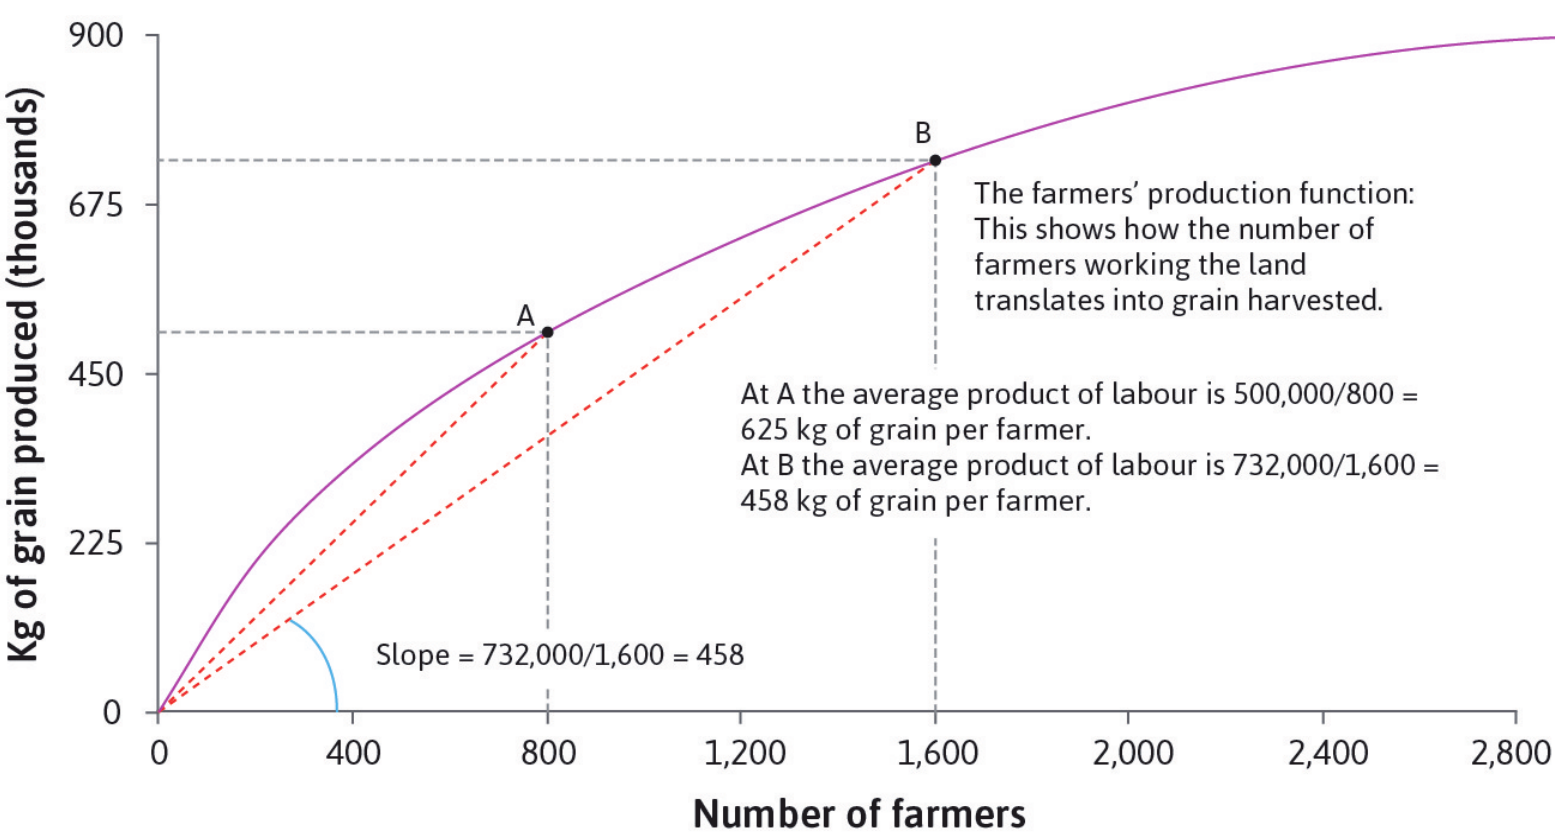
\includegraphics[width=0.8\textwidth]{./figures/production-1.png}
\end{frame}

\begin{frame}[t]{Production (Cont.)}
    Marginal Production of Labor (MPL): $y = f\left( x \right)  \implies MPL = \frac{dy}{dx} = \frac{df\left( x \right) }{dx} $
    \centering
    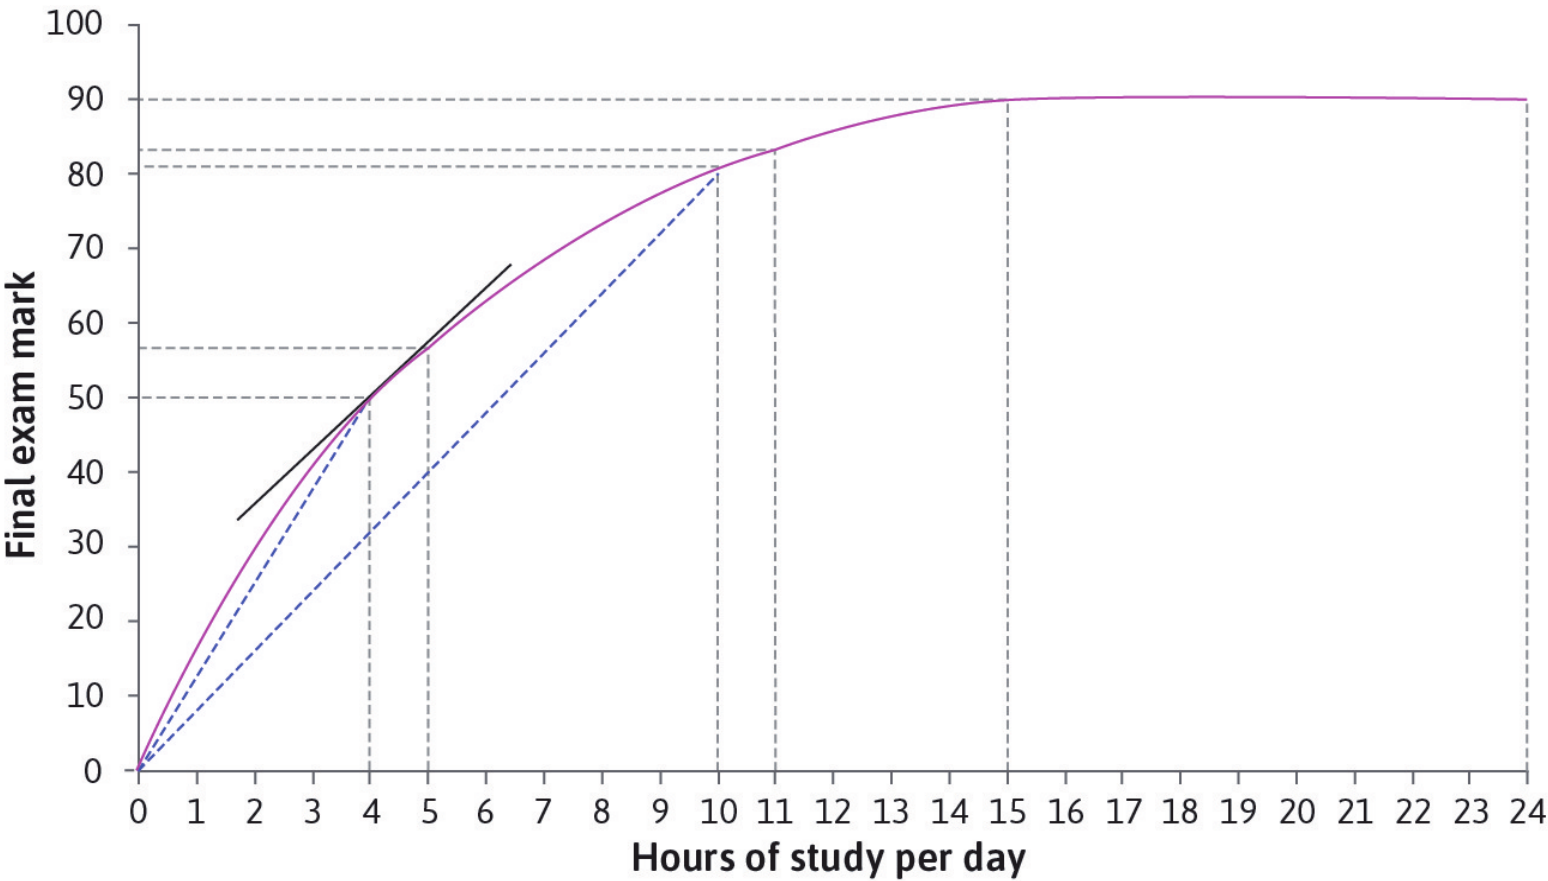
\includegraphics[width=0.8\textwidth]{./figures/production-2.png}

\end{frame}

\begin{frame}[t]{Concave / Convex and Diminishing MPL}
    \begin{columns}
	\begin{column}{0.37\textwidth}
	    \centering
	    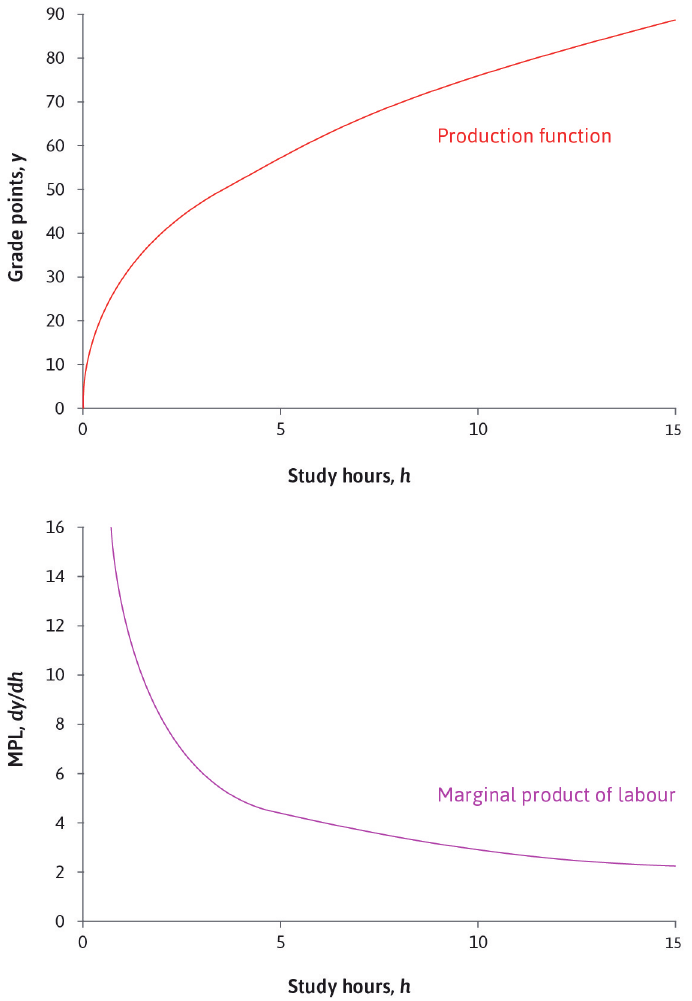
\includegraphics[width=\textwidth]{./figures/production-3.png}
        \end{column}
	\begin{column}{0.63\textwidth}
	    \begin{itemize}
	        \item Concave v.s. Convex: Is production function looks like a ``cave''?
		\item Concave function: whenever study hour increases by 1 unit, the speed of increase in grade point is decreasing.
		\begin{itemize}
		    \item  $\implies $ decreasing MPL
		\end{itemize}
	    \end{itemize}
	\end{column}
    \end{columns}
\end{frame}

\begin{frame}[t]{Application of Differentiation: Elasticity}
    \begin{definition}[The ``A'' Elasticity of ``B'']
	percentage change in ``B'' when ``A'' changes by $1\%$, i.e., $-\frac{\%  \Delta B}{\%  \Delta A} $
    \end{definition}
    \begin{definition}[The price elasticity of quantity demanded]
	percentage change in quantity demanded when price changes by $1\%$, i.e., $-\frac{\%  \Delta Q}{\%  \Delta P} $
    \end{definition}
    \begin{itemize}
	\item Calculate percentage: $\frac{\text{value}}{\text{total amount}}  \times 100 \% $
        \item Expand the $\%  \Delta $ part: $\% \Delta Q = \frac{ \Delta Q}{Q} $
	\item Use differentiation notation: $\% \Delta Q = \frac{ \Delta Q}{Q} = \frac{d Q}{Q}  $
	\item Rewrite Def of elasticity: $-\frac{\%  \Delta Q}{\%  \Delta P} = \left. - \frac{dQ}{Q} \middle/ \frac{dP}{P} \right.  = -\frac{P}{Q} \frac{dQ}{dP} $
    \end{itemize}
\end{frame}

\begin{frame}[standout]{Technological Progress Example: Numerically calculating $ \pi  $}
\label{slide:Example_of_Technological_Progress__Numerically_calculating____pi___}

    --\href{https://www.youtube.com/watch?v=gMlf1ELvRzc}{The Discovery That Transformed Pi} by \href{https://www.youtube.com/channel/UCHnyfMqiRRG1u-2MsSQLbXA}{Veritasium }

\end{frame}




\end{document}
